\documentclass[a4paper, 11pt]{article}

\usepackage[utf8]{inputenc}
\usepackage[english]{babel}
\usepackage[bookmarks=false]{hyperref}
\usepackage{a4wide}
\usepackage{graphicx}
\usepackage{float}
\usepackage{amsmath, amssymb, amsfonts, amsthm}
\usepackage{relsize}
\usepackage{indentfirst}
\usepackage[bottom]{footmisc}
\usepackage[intoc]{nomencl}
\usepackage{nameref}
\usepackage{url}
\usepackage{listings}
\usepackage[normalem]{ulem}
\usepackage{multicol}
\usepackage{setspace}
\usepackage[toc, page]{appendix} 
\usepackage{multirow}

\onehalfspacing

\makenomenclature

\lstset{
    basicstyle=\ttfamily,
    commentstyle=\ttfamily,
    frame=tb, 
    showstringspaces=false,
    captionpos=b
}

\hypersetup{
    pdftitle={Anonymization of Datasets with Privacy, Utility and Risk 
Analysis},
    pdfborder={0 0 0}
}

\title{Privacy Enhancing Technologies \\ [0.8em] \smaller{} Anonymization of 
Datasets with Privacy, Utility and Risk Analysis}
\author{David Capela \and Rui Fernandes}
\date{\today}

\begin{document}

\renewcommand\labelitemi{--}
\renewcommand{\nomname}{Acronyms}
\newcommand{\hlgreen}[1]{{\sethlcolor{green}\hl{#1}}}

\renewcommand{\today}{\ifcase \month\or January\or February\or March\or %
April\or May\or June\or July\or August\or September\or October\or November\or %
December\fi, \number \year}

\begin{titlepage}
    \begin{center}
        \begin{minipage}{.75\linewidth}
            \centering
            
\includegraphics[width=0.5\textwidth]{img/fcup.png}\par\vspace{1cm}
            \vspace{1.5cm}
            \href{https://sigarra.up.pt/fcup/pt/web_page.Inicial}{\scshape\LARGE Faculty of Sciences of the University of Porto} \par
            \vspace{1cm}
            \href{https://msi.dcc.fc.up.pt/}{\scshape\Large Master's Degree in Information Security} \par
            \vspace{1.5cm}
            \maketitle
        \end{minipage}
    \end{center}
    \vspace{2cm}
    \thispagestyle{empty}
    \pagebreak
\end{titlepage}

\pagenumbering{roman}

\begin{abstract}
This report describes the first assignment of the Privacy Enhancing 
Technologies course within the context of the 
\href{https://msi.dcc.fc.up.pt/}{Master's Degree in Information Security} at 
the \href{https://sigarra.up.pt/fcup/pt/web_page.Inicial}{Faculty of Sciences 
of the University of Porto}.

This assignment aims at anonymizing a dataset cointaining personal information 
of individuals while maintaining a reasonable level of data utility. To do so, 
several privacy models were applied, followed by a careful evaluation of the 
re-identification risk and utility metrics as to ensure that an acceptable 
trade-off between privacy protection an utility was achieved considering the 
requirements we defined.

\

\noindent\textbf{Keywords:} Data Anonymization, Privacy Preserving Data Publishing, 
Privacy Models, Privacy-Utility Trade-off
\end{abstract}

\pagebreak

\tableofcontents \pagebreak
\listoffigures \pagebreak
\listoftables
\lstlistoflistings \pagebreak

\nomenclature[01]{PII}{Personally Identifiable Information}
\nomenclature[02]{PPDDM}{Privacy Preserving Distributed Data Mining}
\nomenclature[03]{PPDM}{Privacy Preserving Data Mining}
\nomenclature[04]{PPDP}{Privacy Preserving Data Publishing}
\nomenclature[05]{QID}{Quasi-Identifier}

\printnomenclature

\pagebreak

\pagenumbering{arabic}

\section{Introduction}

Often times, one wants to release data to the public for a variety of reasons -- \textit{e.g.}
to compute some statistics or to perform other data analysis tasks. However,
prior to anonymization, data usually contains sensitive information about
individuals and sharing it could potentially violate their privacy. Privacy
Preserving Data Publishing (PPDP) addresses this issue by providing mechanisms
to ensure privacy protection while maintaining the utility of data.

In this assignment, we perform a detailed analysis of the anonymization process 
of a dataset. To do so, we first start by choosing the dataset to anonymize, 
define the privacy and utility requirements, apply different privacy models 
and, finally, compare the privacy protection and the data utility offered by 
each of them. This being said, is clear that the  challenge does not only lie 
in anonymizing data itself, but also in preserving an acceptable level of 
information utility.

Throughout this report, we explain the reasoning behind the choices made on 
each of the steps of this process.

\subsection*{Document Structure}

The structure of this report is as follows:

\begin{itemize}
    \item Section \ref{sec:import}, \textbf{\nameref{sec:import}}, specifies the
    goal of the release of the anonymized dataset and defines both privacy and 
    utility requirements for the anonymization process.
    \item Section \ref{sec:dataset}, \textbf{\nameref{sec:dataset}}, provides a 
    characterization of the original dataset by classifying attributes and 
    analyzing the re-identification risk.
    \item In Section \ref{sec:privacy}, \textbf{\nameref{sec:privacy}}, we 
    apply different privacy models to the target dataset and analyse the privacy 
    protection and data utility offered by each of them.   
    \item Section \ref{sec:conclusion}, \textbf{\nameref{sec:conclusion}}, 
    concludes the work and suggests future improvements.
\end{itemize}

\pagebreak

\section{Selection, Importing \& Goal of Dataset} \label{sec:import}

In the following section, we describe the dataset, define the privacy and 
utility requirements for the anonymization process and specify the goal with 
which the anonymized dataset would be released.

For this assignemt, we generated our own dataset based on a fictional dataset 
available at 
\url{https://www.kaggle.com/spscientist/students-performance-in-exams}, 
consisting of the scores obtained in tests by high school students from the 
United States, as well as some social and economic aspects.

\subsection{Privacy \& Utility Requirements} \label{sec:requirements}

With the use of anonymization operations, it is inevitable that some 
information will be lost. However, even after the anonymization process, the 
resulting data should preserve an acceptable level of utility. This being said, 
it should still be possible to answer questions along the lines of the 
following:

\begin{itemize}
    \item How does the parental level of education affect one's school 
    performance?
    \item How does one's gender relate to their school performance?
\end{itemize}

On the other hand, when it comes to privacy, the following requirements must be 
met:

\begin{itemize}
    \item Under no circumstances should the re-identification risk be greater 
    than 50\%.
    \item No record in the anonymized dataset should be unique.
\end{itemize}

It is important to clarify that in this context \textit{anonymity} refers to 
the indistinguishably from other records with respect to QID.

\subsection{Data Preprocessing}

In the original dataset, the following attributes are present (see Table 
\ref{tab:before-faker}):

\begin{itemize}
    \item \textbf{Gender}
    \item \textbf{Ethnicity:} This attribute was already subject to anonymization
    in the original dataset. As a matter of fact, the values for this attribute
    are grouped into \texttt{Group A}, \texttt{B}, \texttt{C}, \texttt{D} and
    \texttt{E}.
    \item \textbf{Parental level of education}
    \item \textbf{Lunch:} Wether the student had a standard or a free/reduced 
    lunch.
    \item \textbf{Test preparation course:} Wether or not the student completed 
    a test preparation course.
    \item \textbf{Math, Reading \& Writing score:} These attributes will be 
    combined in a single attribute, \texttt{Average Score}, since we are only 
    interested in the overall school performance and not the performance in 
    specific subjects. The values of the resulting attribute will be in the range 
    $[0, 100]$ and will be calculated according to
    $$\text{Average Score} = \frac{\text{Math Score} + \text{Reading Score} + \text{Writing Score}}{3}$$
    and rounded to the nearest integer.
\end{itemize}

\begin{table}[H]
	\centering
	\begin{tabular}{|l|c|}
		\hline
		\textbf{Number of Records}                &   1000 \\ \hline
		\textbf{Number of Attributes}             &   8    \\ \hline
		\multicolumn{1}{|c|}{\textbf{Attributes}} &   
		\begin{tabular}[c]{@{}c@{}}Gender, Race/Ethnicity, Parental\\ 
        Level of Education, Lunch,\\ Test Preparation Course, Math Score,\\ Reading 
        Score, Writing Score\end{tabular} \\ \hline
	\end{tabular}
	\caption{Characterization of the original dataset}
	\label{tab:before-faker}
\end{table}

Considering the fact that this dataset doesn't include any personally 
identifiable information (PII), we added some identifying attributes and other 
sensitive information -- \textit{i.e.} name, social security number, birth date 
(in the \texttt{yyyy-MM-dd} format) and city -- as to make it more suitable for 
the anonymization process. This was done using \texttt{Faker}, a Python library 
that allows the generation random data (see Listing \ref{lst:faker} and Table 
\ref{tab:after-faker}).\\

\begin{table}[H]
	\centering
	\begin{tabular}{|l|c|}
		\hline
		\textbf{Number of Records}                &   1000 \\ \hline
		\textbf{Number of Attributes}             &   9    \\ \hline
		\multicolumn{1}{|c|}{\textbf{Attributes}} &   
		\begin{tabular}[c]{@{}c@{}}Name, SSN, Birth Date, City, 
        Gender,\\ Race/Ethnicity, Parental Level of\\ Education, Test Preparation 
        Course, \\ Average Score\end{tabular} \\ \hline
	\end{tabular}
	\caption{Characterization of the original dataset after introducing 
    synthetic data}
	\label{tab:after-faker}
\end{table}

\pagebreak

\section{Characterization of the Dataset \& Coding Models} \label{sec:dataset}

In this section, we provide an overview of the original dataset and classify 
attributes into \textit{identifying}, \textit{quasi-identifying}, 
\textit{sensitive} and \textit{insensitive}. Finally, we analyze the 
distribution of data the privacy risks.

As previously stated in Section \ref{sec:import}, this dataset contains the 
scores obtained in tests by high school students. Essentially, it has 1,000 
records, each with 9 attributes, none of which have null values. A more 
in-depth view of the dataset is presented in Table \ref{tab:values-types}, and 
an excerpt is presented in Figure \ref{fig:input-data}.

\vspace{3\baselineskip}

\begin{table}[H]
	\centering
	\begin{tabular}{|c|c|c|}
		\hline
		\textbf{Attribute}                          &         
		\textbf{Possible Values}                                                        
		                                            &         
		\textbf{Type} \\ \hline
		Name                                        & US      
		Names (first and last name)                                                     
		                                                                                
		                                            & String  \\ \hline
		SSN                                         &         
		\begin{tabular}[c]{@{}c@{}}9 digit numbers in the format\\ 
		\texttt{AAA-GG-SSSS}\end{tabular}                                               
		                                            & String  \\ \hline
		Gender                                      &         
		Male/Female                                                                     
		                                            & String  
		\\ \hline
		City                                        & US      
		Cities                                                                          
		                                            & String  
		\\ \hline
		Birth Date                                  &         
		\begin{tabular}[c]{@{}c@{}}Values in the format \texttt{yyyy-MM-dd}\\ ranging 
		from 2002-01-01 to                          &         \\ 2005-01-01\end{tabular}                                & 
		DateTime      \\ \hline
		Race/Ethnicity                              & Group   
		\texttt{A}, \texttt{B}, \texttt{C}, \texttt{D} or \texttt{E}                    
		                                                                                
		                                            & String  \\ \hline
		\begin{tabular}[c]{@{}c@{}}Parental Level   &         \\ of Education\end{tabular} & 
		\begin{tabular}[c]{@{}c@{}}Some High School, High School,\\ Some College, 
		Associate's Degree,                         &         \\ Bachelor's Degree, Master's Degree,\end{tabular} & String 
		\\ \hline
		\begin{tabular}[c]{@{}c@{}}Test Preparation &         \\ Course\end{tabular}     & 
		Completed, None                                                                 
		                                            & String  
		\\ \hline
		Average Score                               & {[}0,   
		100{]}                                                                          
		                                            & Integer \\ 
		\hline
	\end{tabular}
	\caption{Possible values and type for each attribute}
	\label{tab:values-types}
\end{table}

\pagebreak

Next, we import the dataset into ARX (Fig. \ref{fig:import-data}), an open 
source data anonymization tool developed in Java that supports several privacy 
models such as $k$-anonymity, $\ell$-diversity $t$-closeness and differential 
privacy, as well as utility metrics for analyzing data utility and 
re-identification risks.

\begin{figure}[H]
    \centering
    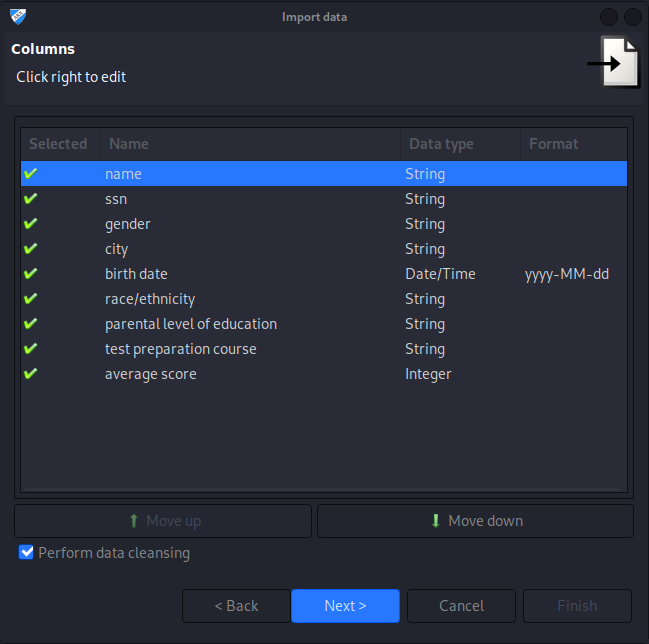
\includegraphics[width=.7\textwidth]{img/import-data.png}
    \caption{Importing data into ARX}
    \label{fig:import-data}
\end{figure}

\begin{figure}[H]
    \centering
    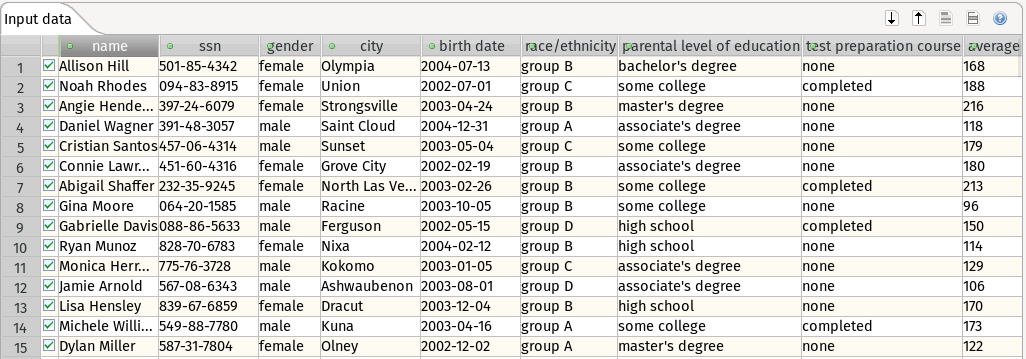
\includegraphics[width=\textwidth]{img/input-data.png}
    \caption{Excerpt of the dataset}
    \label{fig:input-data}
\end{figure}

\pagebreak

\subsection{Distribution of Data for Each Attribute}

Given the nature of the data, it is crucial to ensure that it follows a 
reaseonable distribution. To do so, we analyzed the summary statistics and 
distribution for each attribute using ARX, as presented in Figures 
\ref{fig:name-arx} to \ref{fig:score-distr}.\\

\begin{figure}[H]
    \centering
    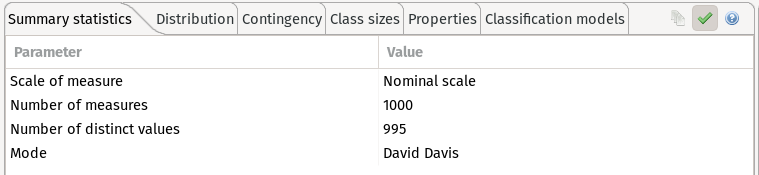
\includegraphics[width=.9\textwidth]{img/name.png}
    \caption{Summary statistics for the \texttt{Name} attribute}
    \label{fig:name-arx}
\end{figure}

\vspace{2\baselineskip}

\begin{figure}[H]
    \centering
    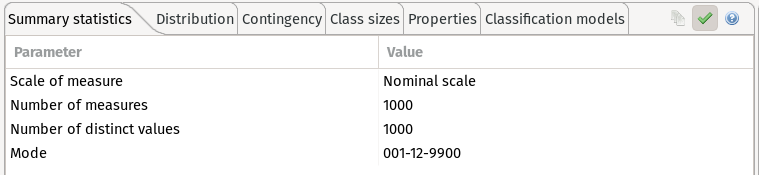
\includegraphics[width=.9\textwidth]{img/ssn.png}
    \caption{Summary statistics for the \texttt{SSN} attribute}
\end{figure}

\vspace{2\baselineskip}

\begin{figure}[H]
    \centering
    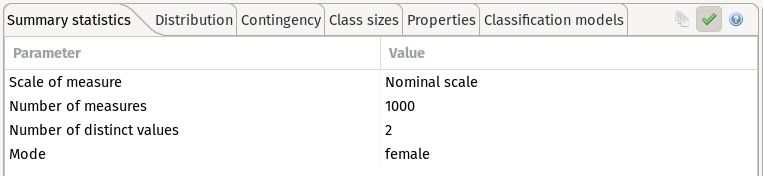
\includegraphics[width=.9\textwidth]{img/gender.png}
    \caption{Summary statistics for the \texttt{Gender} attribute}
\end{figure}

\begin{figure}[H]
    \centering
    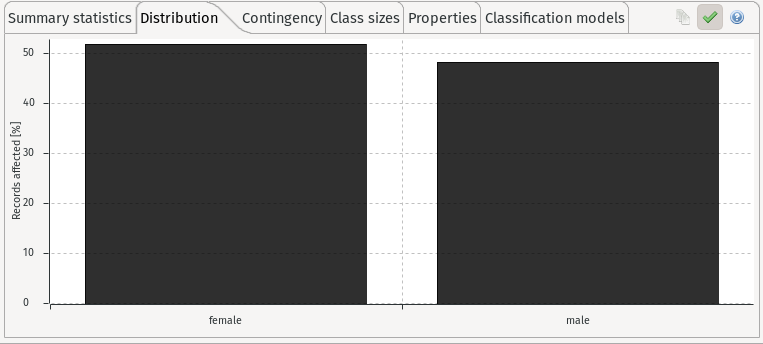
\includegraphics[width=.9\textwidth]{img/gender-distr.png}
    \caption{Distribution of values for the \texttt{Gender} attribute}
\end{figure}

\begin{figure}[H]
    \centering
    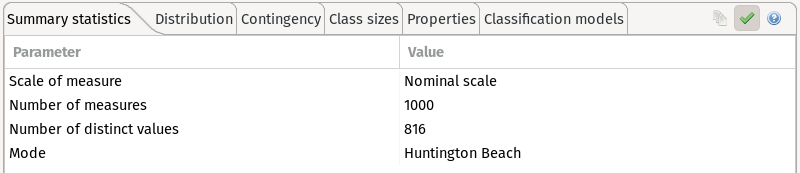
\includegraphics[width=.9\textwidth]{img/city.png}
    \caption{Summary statistics for the \texttt{City} attribute}
\end{figure}

\begin{figure}[H]
    \centering
    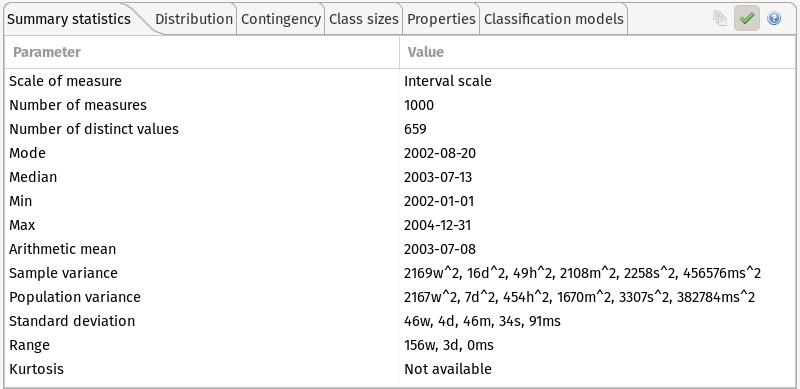
\includegraphics[width=.9\textwidth]{img/birth-date.png}
    \caption{Summary statistics for the \texttt{Date of Birth} attribute}
\end{figure}

\begin{figure}[H]
    \centering
    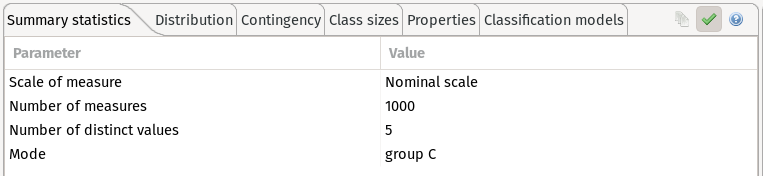
\includegraphics[width=.9\textwidth]{img/race.png}
    \caption{Summary statistics for the \texttt{Race/Ethnicity} attribute}
\end{figure}

\vspace{1.5\baselineskip}

\begin{figure}[H]
    \centering
    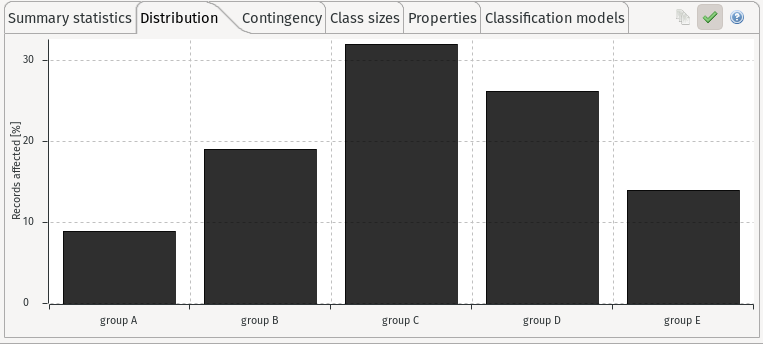
\includegraphics[width=.9\textwidth]{img/race-distr.png}
    \caption{Distribution of values for the \texttt{Race/Ethnicity} attribute}
\end{figure}

\vspace{1.5\baselineskip}

\begin{figure}[H]
    \centering
    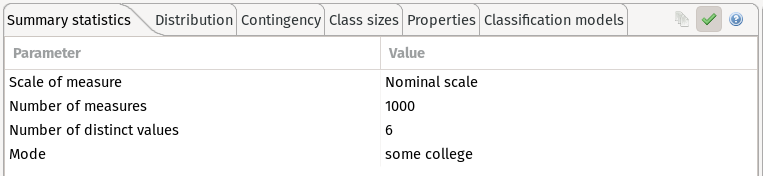
\includegraphics[width=.9\textwidth]{img/education.png}
    \caption{Summary statistics for the \texttt{Parental Level of Education} 
attribute}
\end{figure}

\begin{figure}[H]
    \centering
    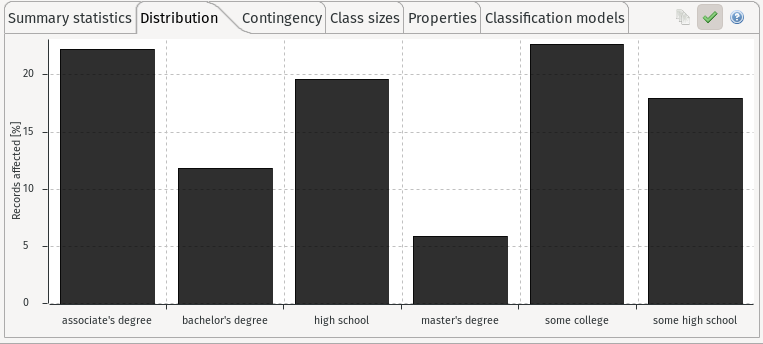
\includegraphics[width=.9\textwidth]{img/education-distr.png}
    \caption{Distribution of values for the \texttt{Parental Level of 
Education} attribute}
\end{figure}

\begin{figure}[H]
    \centering
    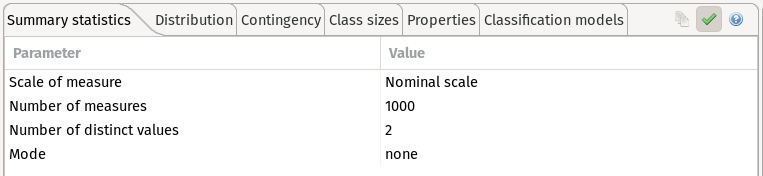
\includegraphics[width=.9\textwidth]{img/test-preparation.png}
    \caption{Summary statistics for the \texttt{Test Preparation Course} 
attribute}
\end{figure}

\begin{figure}[H]
    \centering
    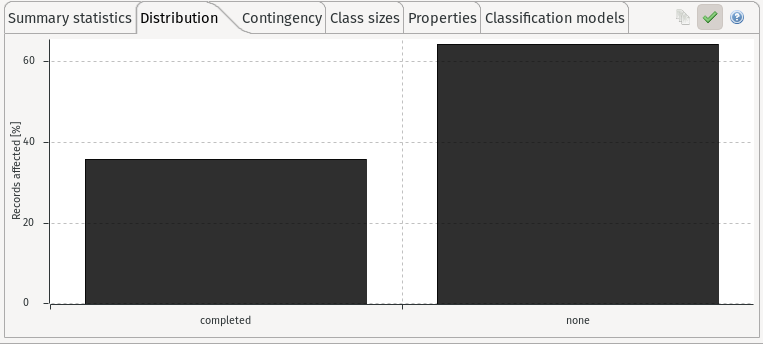
\includegraphics[width=.9\textwidth]{img/course-distr.png}
    \caption{Distribution of values for the \texttt{Test Preparation Course} 
attribute}
\end{figure}

\begin{figure}[H]
    \centering
    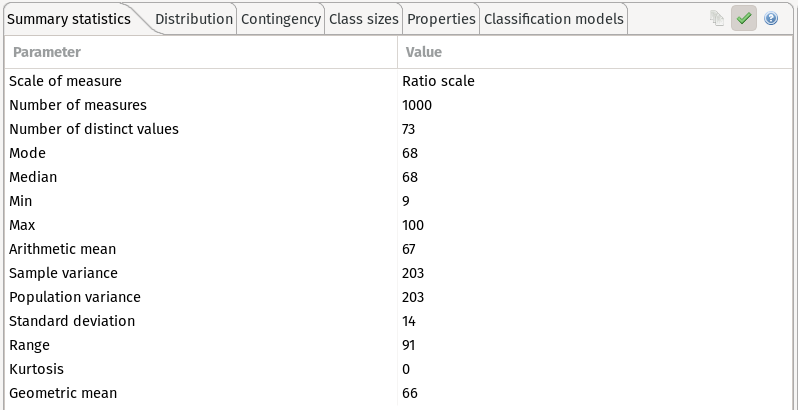
\includegraphics[width=.9\textwidth]{img/score.png}
    \caption{Summary statistics for the \texttt{Average Score} attribute}
\end{figure}

\vspace{6\baselineskip}

\begin{figure}[H]
    \centering
    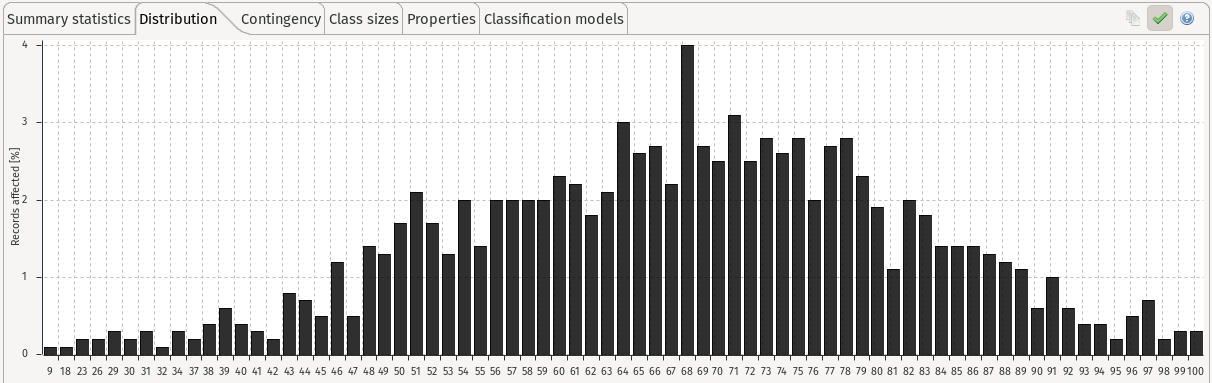
\includegraphics[width=\textwidth]{img/score-distr.png}
    \caption{Distribution of values for the \texttt{Average Score} attribute}
    \label{fig:score-distr}
\end{figure}

\pagebreak

\subsection{Classification of Attributes}

The attributes can be classified as follows:

\begin{itemize}
    \item \textbf{Identifying Attributes:} Name, SSN. As any real world 
    scenario, more than one student have the same name. Identifying Attributes
    are associated with a high risk of re-identification and, as such, they will
    be removed before disclosing the dataset.
    \item \textbf{Quasi-Identifiers:} Birth Date, City, Gender, Race/Ethnicity.
    These attributes do not explicitly identify a record owner but can be combined 
    with data from public sources in an attempt to de-anonymize the owner of a 
    record.
    \item \textbf{Insensitive Attributes:} Parental Level of Education, Test 
    Preparation. These attributes do not pose any privacy risks and, as such, they 
    will be kept unmodified.
    \item \textbf{Sensitive Attributes:} Average Score. As any sensitive 
    attribute, its disclosure may be undesirable from the record owner standpoint 
    and, as such, it will be kept unmodified but will be subject to restrictions 
    imposed by the privacy model -- \textit{e.g.} $l$-diversity, $t$-closeness, etc.
\end{itemize}

\vspace{\baselineskip}

We were particularly careful when differentiating quasi-identifiers from 
sensitive attributes because a wrong classification may result in a lower 
privacy protection -- and hence a higher re-identification risk -- than what 
was expected. As a matter of fact, incorrectly classifying an attribute as a 
quasi-identifier will result in a greater loss of information due to the 
anonymization operations that will be applied to each QID. On the other hand, 
misclassifying an attribute as a quasi-identifier when it is, in fact, a 
sensitive attribute can have an undesirable effect on the privacy protection in 
the sense that an attacker is then able perform an attribute linkage attack.

The classification of the attributes can be checked in ARX (Figs. 
\ref{fig:arx-qid-1} and \ref{fig:arx-qid-2}) -- high values of 
distinction\footnote{Distinction measures the degree to which variables make 
records distinct.} and separation\footnote{Separation measures the degree to 
which combinations of variables separate the records.} indicate 
\uline{probable} QIDs.

\begin{figure}[H]
	\centering
	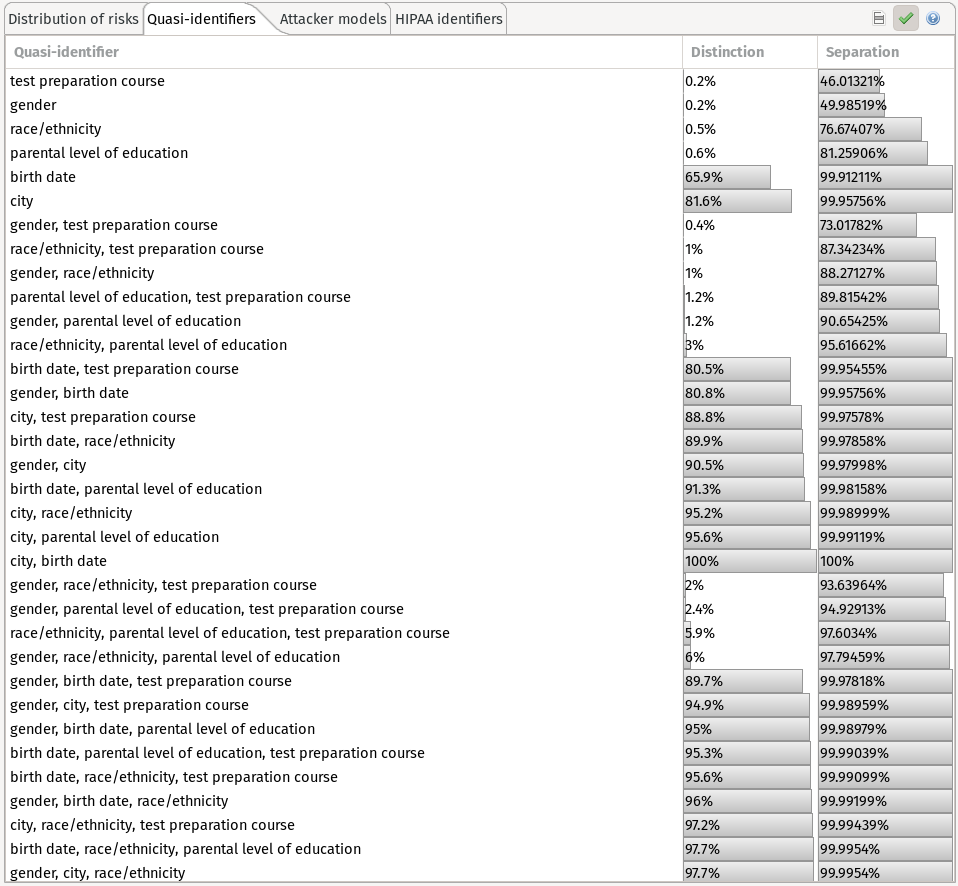
\includegraphics[width=\textwidth]{img/qid-1.png}
	\caption{Identification of QIDs through ARX (i)}
	\label{fig:arx-qid-1}
\end{figure}

\begin{figure}[H]
	\centering
	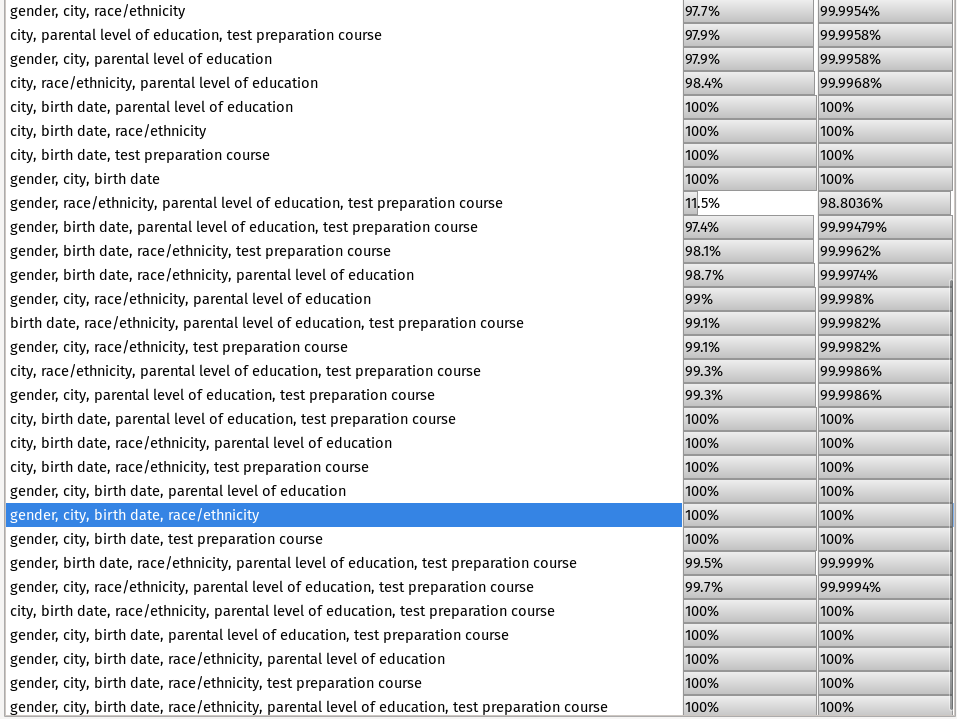
\includegraphics[width=\textwidth]{img/qid-2.png}
	\caption{Identification of QIDs through ARX (ii)}
	\label{fig:arx-qid-2}
\end{figure}

\pagebreak

\subsection{Risk Analysis} \label{sec:risk-analysis}

Figure \ref{fig:arx-risk} shows an overview of several measures for 
re-identification risks considering three different attacker models -- the 
prosecutor attacker model, the journalist attacker model, and the marketer 
attacker model.

In the prosecutor scenario, an attacker targets a specific individual and knows 
whether or not they are in the dataset; in the journalist scenario, an 
adversary selects a target at random because the re-identification of any 
record achieves the purpose; and finally, in the marketer scenario, an attacker 
targets as many individuals as possible, which means that an attack is 
considered successful if a considerable portion of the records can be 
re-identified.

As we can see, regardless of the attacker model we consider, the values for the 
re-identification risk are very close to 100\%. This is highlighted by the fact 
that the birth date uniquely identifies 65.9\% of the records; furthermore, the 
combination of the birth date and the ethnicity is enough to uniquely identify 
89.9\% of the records.\\

\begin{figure}[H]
    \centering
    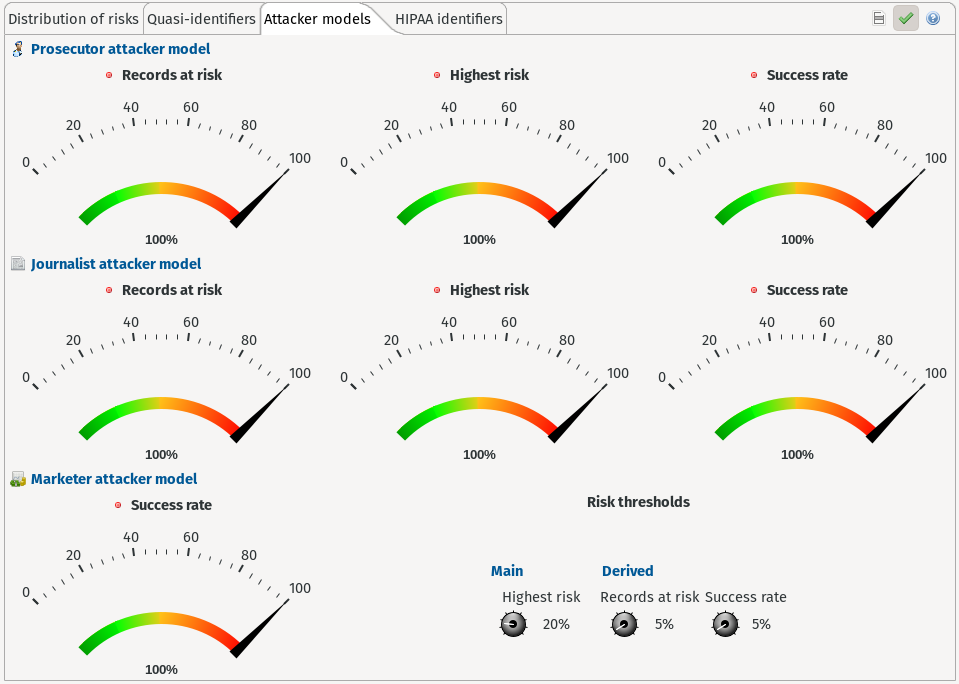
\includegraphics[width=.9\textwidth]{img/risk.png}
    \caption{Risk of re-identification on each attacker model}
    \label{fig:arx-risk}
\end{figure}

In order to reduce the re-identification risk, we applied different privacy 
models to the data, which we will describe in the following sections.

\pagebreak

\section{Privacy Models} \label{sec:privacy}

In an anonymization process, the first thing to do is removing PII before 
disclosing the dataset. PII includes but is not limited to:

\begin{multicols}{2}
\begin{itemize}
    \item Name
    \item Personal identification numbers such as social security number, 
passport number, driver's license number, credit card number, etc.

    \item Telephone number
    \item Email address
    \item Biometric data
\end{itemize}
\end{multicols}

However, simply removing PII from the dataset is not sufficient because an 
adversary can use background knowledge and cross-correlation with other 
databases to re-identify individual records. A famous example of such kind of 
attack includes the de-anonymization of a Massachusetts hospital discharge 
database, carried out by Latanya Sweeney, who joined it with a public voter 
database and then used the combination of both to determine the values of 
medical attributes for each person who appeared in both databases 
\cite{sweeney_2021}.

\subsection{Model 1: $k$-Anonimity \& $\ell$-Diversity}

$k$-Anonymity requires that each record in the dataset must be 
indistinguishable from at least $k - 1$ other records with respect to every 
quasi-identifier \cite{Sweeney2002kAnonymityAM}. In other words, these $k$ 
records form an \textit{equivalence class} such that the minimum equivalence 
class size is $k$. As a result, the probability of linking a record owner to 
its record is at most $1/k$.

However, it is important to note $k$-anonimity alone does not ensure privacy as 
it assumes that each record represents a distinct record owner. However, if 
more than one record refers to the same individual, a set of $k$ records will 
represent fewer than $k$ individuals, which causes a record owner to be 
under-protected because the probability of re-identification will be greater 
than $1/k$ \cite{10.5555/1855031}. Even though this is not a problem in this 
dataset as each record belongs to a different individual, it is something worth 
keeping in mind since it allows for homogeneity attacks as well as background 
knowledge attacks \cite{Machanavajjhala2006LdiversityPB}.

On the other hand, $\ell$-diversity addresses the limitations of $k$-anonymity 
by requiring that each equivalence class to have at least $\ell$ distinct 
records. This encompasses the idea that a sensitive attribute must be "diverse" 
within each equivalence class. 

\pagebreak

In the first privacy model, we applied $k$-anonymity, with $k = 3$ and distinct 
$\ell$-diversity, with $\ell = 2$. In this case, we applied a character masking 
so the gender of the given individual stays anonymous (Fig. 
\ref{fig:gender-model1}), replaced each city with the corresponding 
State\footnote{This transformation was made using a Python script (see Listing 
\ref{lst:city-state}) prior to importing the dataset into ARX.} (Fig. 
\ref{fig:city-model1}), replaced the date of birth with the most generalized 
date interval in the hierarchy defined in Figure \ref{fig:birth-model1} and, 
finally, we kept ethnicity  attribute unmodified due to the fact that it was 
already generalized in the initial dataset.

This is summarized in Table \ref{tab:qid-transformation-model1}:\\

\begin{table}[H]
	\centering
	\begin{tabular}{|c|c|c|}
		\hline
		\textbf{Quasi-identifier} & \textbf{Transformation}          &   
		\textbf{Levels} \\ \hline
		Gender                    & Generalization -- Character masking 
		& 0--1            \\ \hline
		City                      & Generalization -- Class grouping &   
		0--1             \\ \hline
		Birth Date                & Generalization -- Date intervals &   
		0--3             \\ \hline
		Race/Ethnicity            & None                             &   
		0              \\ \hline
	\end{tabular}
	\caption{Transformations applied to each of the QID}
	\label{tab:qid-transformation-model1}
\end{table}

\begin{figure}[H]
	\centering
	
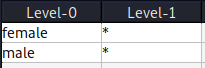
\includegraphics[width=.35\textwidth]{img/qids-trans/qid-model1-gender.png}
	\caption{Gender transformation levels}
	\label{fig:gender-model1}
\end{figure}

\begin{figure}[H]
	\centering
	
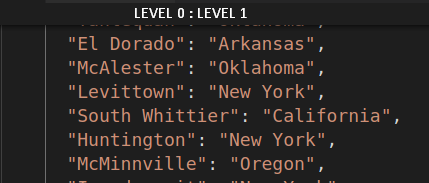
\includegraphics[width=.55\textwidth]{img/qids-trans/qid-model1-city.png}
	\caption{City transformation levels}
	\label{fig:city-model1}
\end{figure}

\begin{figure}[H]
	\centering
	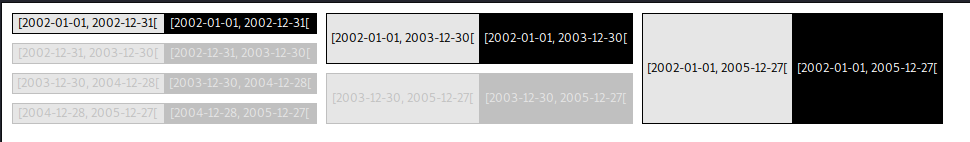
\includegraphics[width=\textwidth]{img/qids-trans/qid-model1-birth.png}
	\caption{Generalization hierarchy for the \texttt{Birth Date} attribute}
	\label{fig:birth-model1}
\end{figure}


\subsubsection{Results}

Applying the transformation specified in Table 
\ref{tab:qid-transformation-model1} with levels $[1, 1, 3, 0]$, we obtained the 
following results:

\vspace{1.5\baselineskip}

\begin{figure}[H]
	\centering
	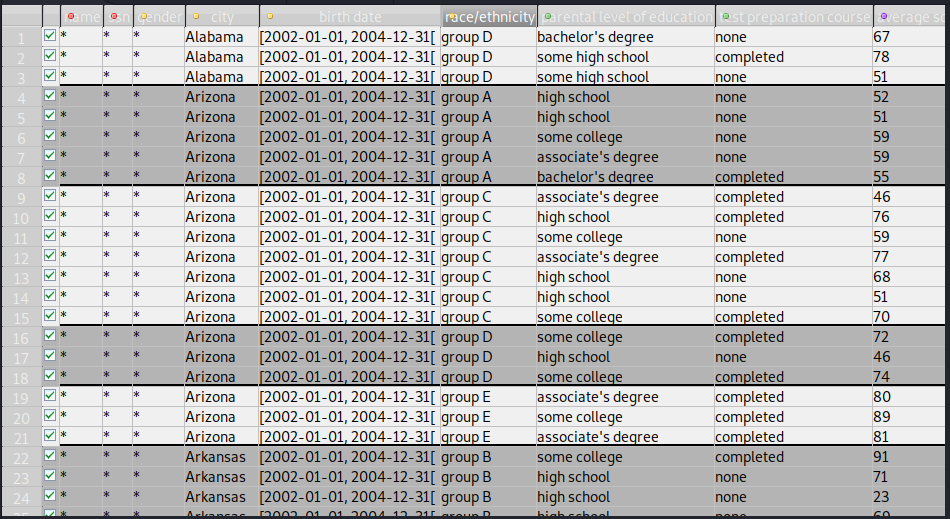
\includegraphics[width=\textwidth]{img/model1-output-data.png}
	\caption{Excerpt of the dataset anonymized with \texttt{Model 1}}
	\label{fig:model1-output}
\end{figure}

\vspace{1.5\baselineskip}

\begin{table}[H]
\centering
\begin{tabular}{|lc|}
\hline
\multicolumn{2}{|c|}{\begin{tabular}[c]{@{}c@{}}\texttt{Model 1}: $k$-Anonimity 
\& $\ell$-Diversity\\ ($k=3, \ell=2$)\end{tabular}} \\ \hline
\multicolumn{1}{|l|}{\textbf{Number of suppressed records}}  & 113  \\ \hline
\multicolumn{1}{|l|}{\textbf{Minimal Class Size}}            & 3    \\ \hline
\multicolumn{1}{|l|}{\textbf{Average Class Size}}            & 8    \\ \hline
\multicolumn{1}{|l|}{\textbf{Maximal Class Size}}            & 42   \\ \hline
\multicolumn{1}{|l|}{\textbf{Number of Classes }}            & 109   \\ \hline
\end{tabular}
\caption{General results after anonymizing with \texttt{Model 1}}
\label{tab:class-size-model1}
\end{table}

\pagebreak

\subsubsection{Risk Analysis \& Data Utility}

Despite the considerably lower re-identification risk when compared to the 
original dataset (see Fig. \ref{fig:risk-model1}), the results we obtained 
using this privacy model were not considered satisfactory, given the 
generalization level of many of the attributes, as well as due to a significant 
loss in quality of data we considered as priority.

Even after the application of the privacy model, it is still possible to answer 
the first question we set as requirements in Section \ref{sec:requirements} -- 
\textit{How does the parental level of education affect one's school 
performance?}. As a matter of fact, since we considered the \texttt{Parental 
Level of Education} as an insensitive attribute, it won't be subject to any 
anonymization operation and, as a result, all the information that relates it 
to the sensitive attribute \texttt{Average Score} will be preserved. However, 
we note that since the \texttt{Gender} attribute was suppressed, all the 
information associated with it will be lost and, as such, the second question 
set as an utility requirement -- \textit{How does one's gender relate to their 
school performance?} -- becomes impossible to answer based on the anonymized 
version of the dataset.\\

\begin{figure}[H]
	\centering
	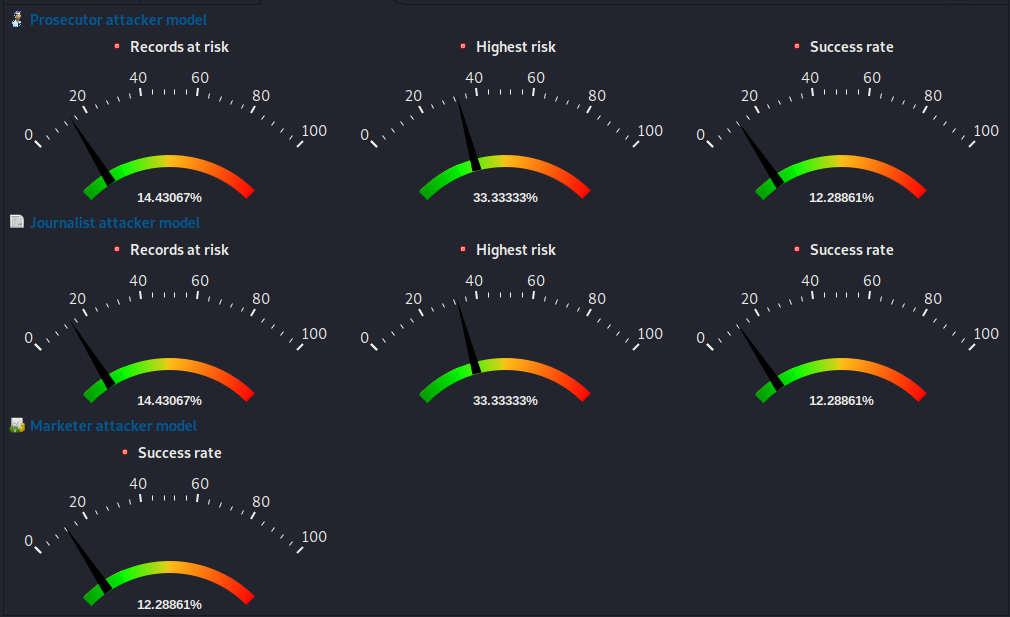
\includegraphics[width=.9\textwidth]{img/risk-model1.png}
	\caption{Risk associated with each attacker model considering \texttt{Model 1}}
	\label{fig:risk-model1}
\end{figure} 

To address this limitation, we experimented with different attribute weights 
for mitigating information loss on QIDs. Thus, we consider another privacy 
model, described in Section {\ref{sec:model2}}, in which preserve the 
\texttt{Gender} attribute in the anonymized version of the dataset and apply a 
higher level of generalization to the \texttt{City} and \texttt{Birth Date} 
attributes.

\pagebreak

\subsection{Model 2: $k$-anonymity and $\ell$-diversity with attribute weights} 
\label{sec:model2}

Based on limitations we identified in the previous model, we now consider a new 
privacy model in which we will again apply $k$-anonymity and $\ell$-diversity, 
with $k = 3$ and $\ell = 2$. However, in order to be able to answer to the 
second question we set as an utility requirement -- \textit{How does one's 
gender relate to their school performance?} -- we made the following 
alterations to the previous privacy model:

\begin{itemize}
    \item Set the \uline{supression limit} to 50\% (see Fig \ref{fig:model2-sl}).
    This limits the maximum numbers records ARX can supress.
    \item In the \uline{coding model}, adjust the trade-off between suppression 
    and generalization (see Fig \ref{fig:model2-cm}). In this case we chose to have 
    slightly more generalization than suppression.
    \item Increase the attribute weight for the \texttt{Gender} (see Fig. \ref{fig:model2-aw}).
    This leads to less information loss on this attribute, which, in turn, makes
    it possible to answer to the second question set as an utility requirement -- \textit{How
    does one's gender relate to their school performance?}
\end{itemize}

\begin{figure}[H]
	\centering
	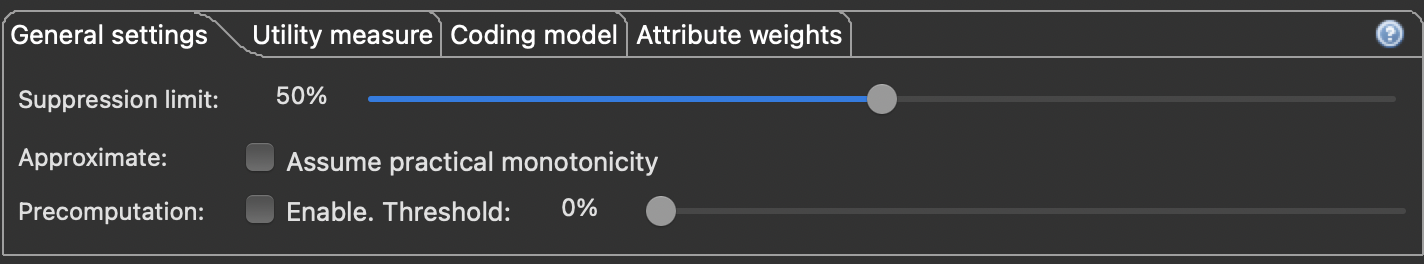
\includegraphics[width=.9\textwidth]{img/supression-limit-model2.png}
	\caption{Supression limit for \texttt{Model 2}}
	\label{fig:model2-sl}
\end{figure}

\begin{figure}[H]
	\centering
	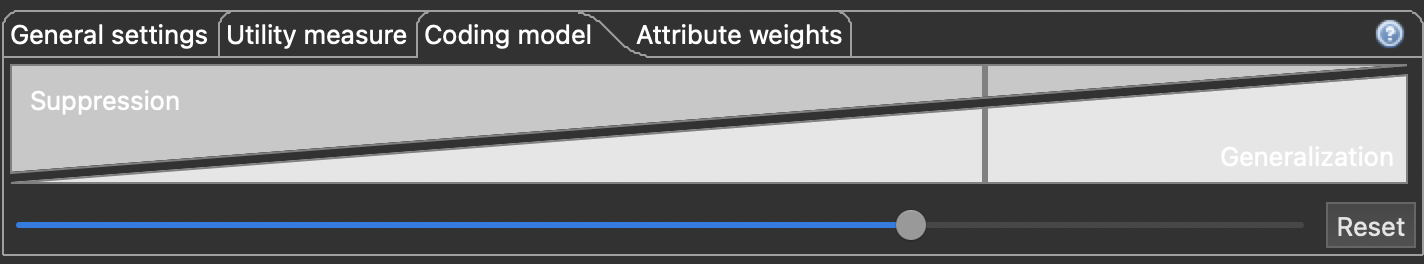
\includegraphics[width=.9\textwidth]{img/coding-model-model2.png}
	\caption{Coding model for \texttt{Model 2}}
	\label{fig:model2-cm}
\end{figure}

\begin{figure}[H]
	\centering
	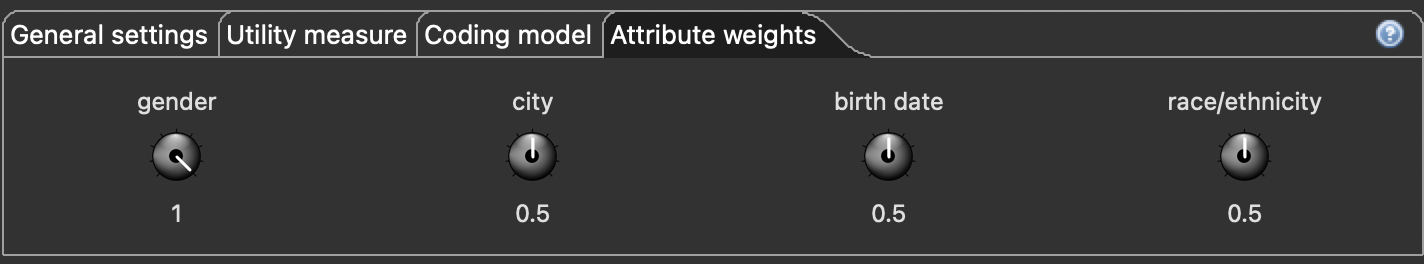
\includegraphics[width=.9\textwidth]{img/attribute-weights-model2.png}
	\caption{Attribute weights for \texttt{Model 2}}
	\label{fig:model2-aw}
\end{figure}

\subsubsection{Results}

Using the same attribute transformations specified in Table 
\ref{tab:qid-transformation-model1}, but now considering the levels $[0, 1, 2, 0]$
and the attribute weights specified in Figure \ref{fig:model2-aw}, the anonymized
dataset is as follows:\\

\begin{figure}[H]
	\centering
	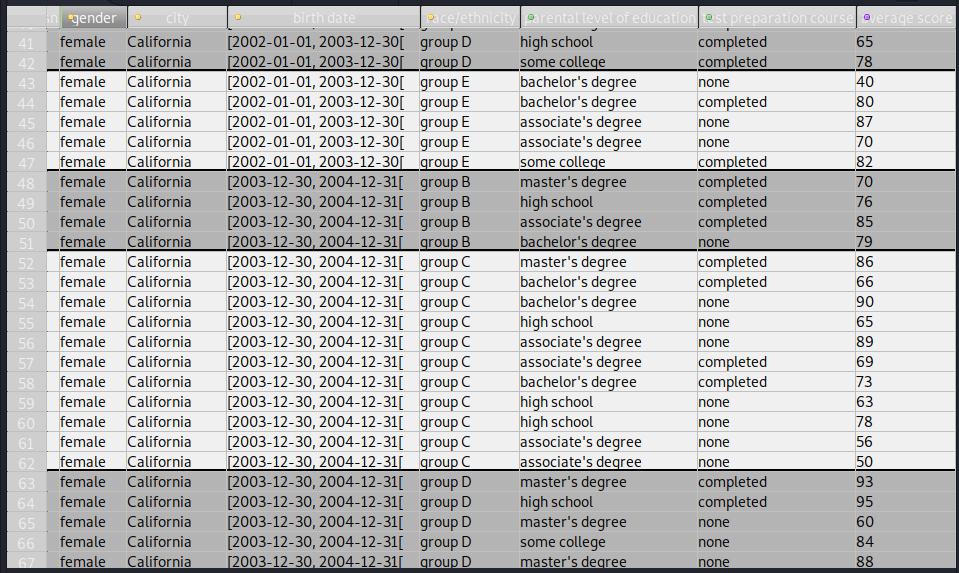
\includegraphics[width=\textwidth]{img/model2-output.png}
	\caption{Excerpt of the dataset anonymized with \texttt{Model 2}}
	\label{fig:model2-output}
\end{figure}

\vspace{2\baselineskip}

\begin{table}[H]
\centering
\begin{tabular}{|lc|}
\hline
\multicolumn{2}{|c|}{\begin{tabular}[c]{@{}c@{}}\texttt{Model 2:} $k$-Anonimity 
\& $\ell$-Diversity\\ ($k=3, \ell=2$, with attribute weights)\end{tabular}} \\ 
\hline
\multicolumn{1}{|l|}{\textbf{Number of suppressed records}} & 454               
       \\ \hline
\multicolumn{1}{|l|}{\textbf{Minimal Class Size}}           & 3                 
       \\ \hline
\multicolumn{1}{|l|}{\textbf{Average Class Size}}           & 4.92              
       \\ \hline
\multicolumn{1}{|l|}{\textbf{Maximal Class Size}}           & 16                
       \\ \hline
\multicolumn{1}{|l|}{\textbf{Number of Classes}}            & 
\multicolumn{1}{l|}{111} \\ \hline
\end{tabular}
\caption{General results after anonymizing with \texttt{Model 2}}
\label{tab:class-size-model2}
\end{table}


\subsubsection{Risk Analysis \& Data Utility}

Considering the limitations of the previous privacy model, \texttt{Model 2} 
takes into account the fact that we must keep information about the 
\texttt{Gender} attribute. As a result of the increase in data utility, the 
number of records at risk increased, as expected.

Besides, the average class size decreased from 8 to 4.92, about half the size 
of the previous model, which may have a significant impact on the privacy 
protection offered, since each record is now, on average, indistinguishable 
from other 3.92 instead of the previous 7. In addition, 454 records, which 
eqautes to about 45\% of the records in the dataset, were suppressed, numbers 
that we considered completely unacceptable. This is even more relevant 
considering that, in an ideal scenario, the dataset should still retain enough 
utilty to so that it can be used for other tasks than the initial.\\

\begin{figure}[H]
	\centering
	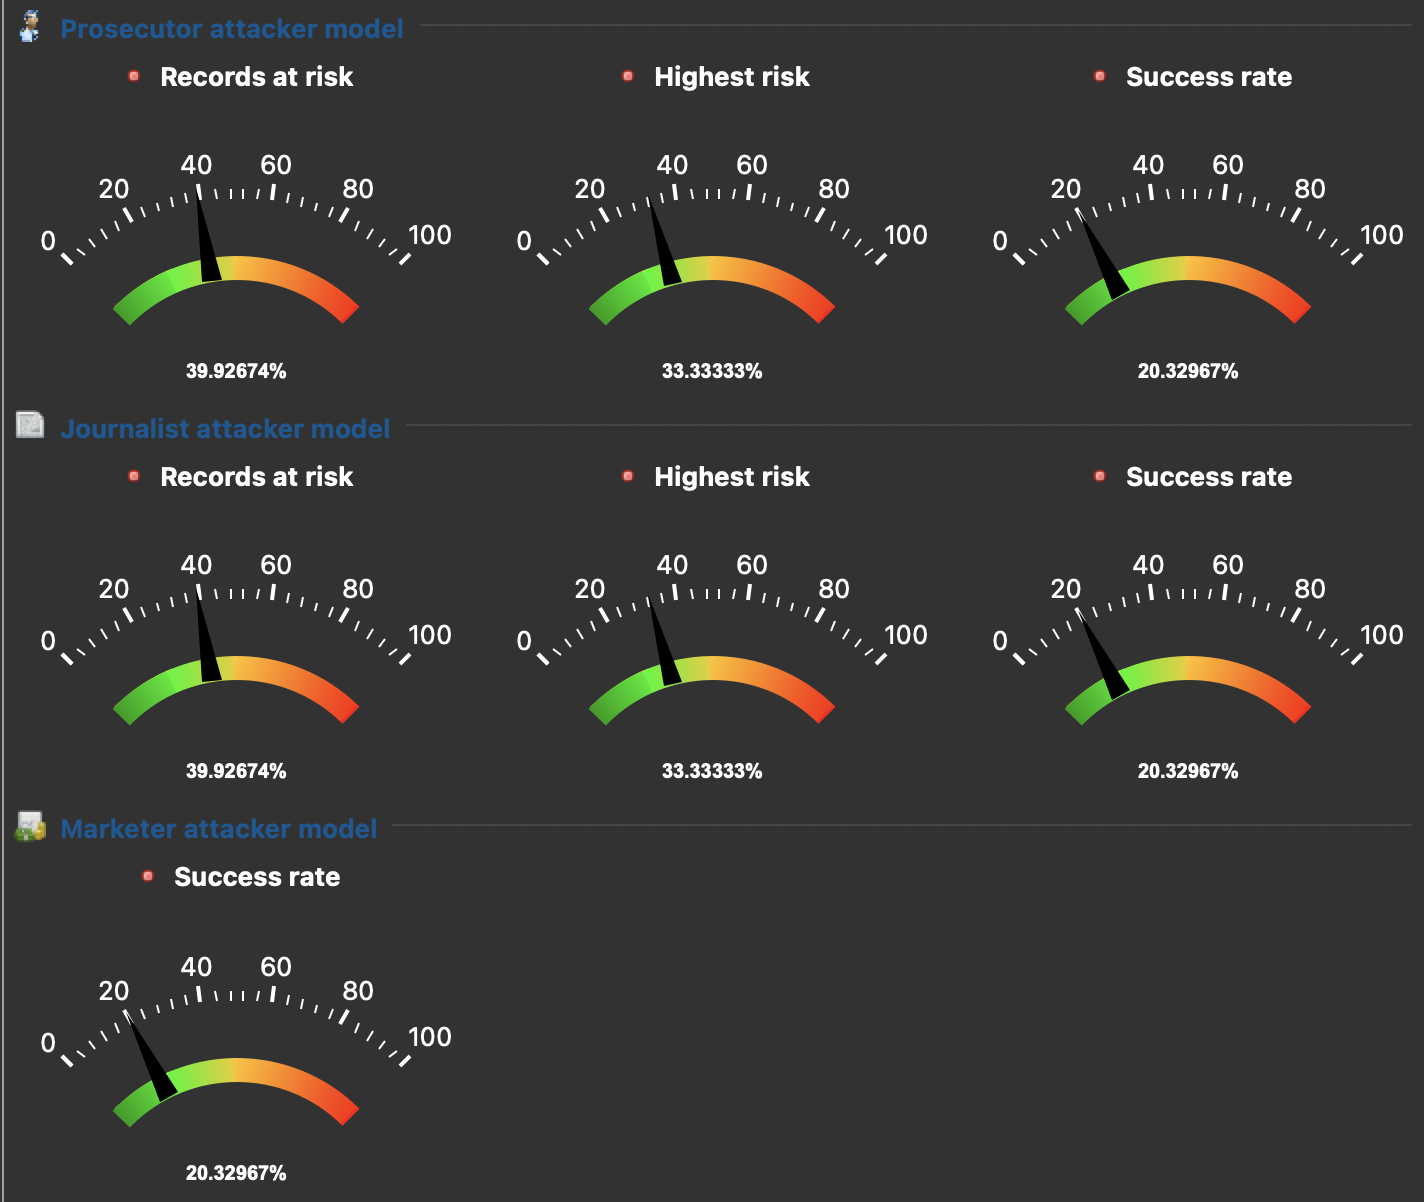
\includegraphics[width=.9\textwidth]{img/risk-model2.png}
	\caption{Risk for \texttt{Model 2}}
	\label{fig:model2-risk}
\end{figure}

\pagebreak

\subsection{Model 3: $t$-Closeness and $k$-Anonymity}

When we applied the previous privacy model, \texttt{Model 2}, too much 
information was lost. In order to avoid this issue, we now consider another 
model, in which we consider $k$-anonymity, with $k=3$ and $t$-closeness, with a 
threshold of 1. With $t$-closeness, we try to achieve a closer distribution of 
sensitive values -- in this case, the \texttt{Average Score} -- in each 
equivalence classes to the initial dataset.

\subsubsection{Results}

Once again, after applying the transformation specified in Table 
\ref{tab:qid-transformation-model1}, this time with levels $[0,1,3,0]$, we 
obtained the following results:

\begin{figure}[H]
	\centering
	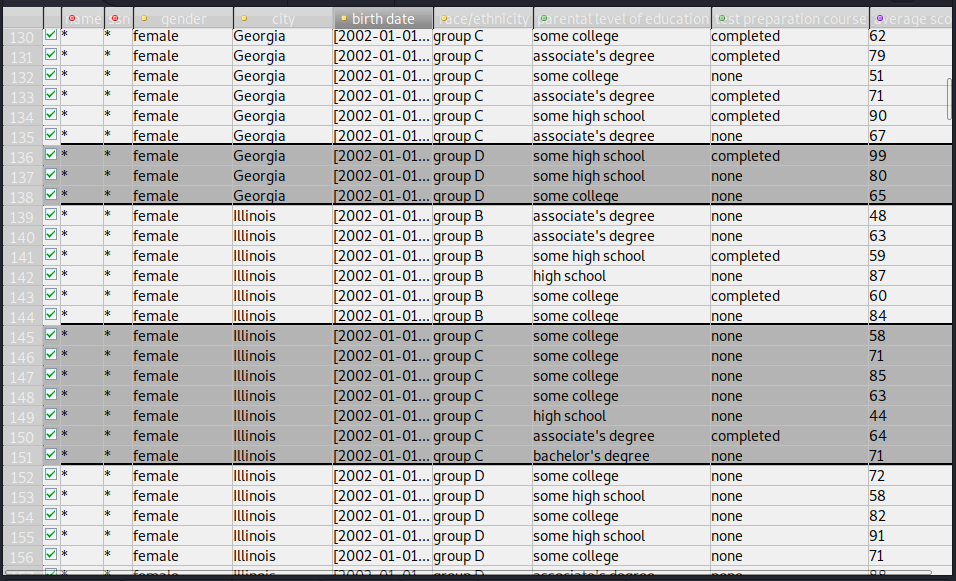
\includegraphics[width=\textwidth]{img/output-model3.png}
	\caption{Anonymized dataset for \texttt{Model 3}}
	\label{fig:model3-output}
\end{figure}

\begin{table}[H]
\centering
\begin{tabular}{|lc|}
\hline
\multicolumn{2}{|c|}{\begin{tabular}[c]{@{}c@{}}\texttt{Model 3:}  
$k$-Anonimity \& $t$-Closeness\\ ($k=3, t=1$)\end{tabular}} \\ \hline
\multicolumn{1}{|l|}{\textbf{Number of suppressed records}} & 235  \\ \hline
\multicolumn{1}{|l|}{\textbf{Minimal Class Size}}           & 3    \\ \hline
\multicolumn{1}{|l|}{\textbf{Average Class Size}}           & 5.71 \\ \hline
\multicolumn{1}{|l|}{\textbf{Maximal Class Size}}           & 27   \\ \hline
\multicolumn{1}{|c|}{\textbf{Number of Classes}}            & 134  \\ \hline
\end{tabular}
\caption{General results after anonymizing with Model 3}
\label{tab:class-size-model3}
\end{table}

\subsubsection{Risk Analysis \& Data Utility}

Similar to \texttt{Model 2}, the resulting dataset is able to answer the two 
questions set as utility requirements since it does not suppress the 
\texttt{Gender} attribute nor the \texttt{Parental Level of Education}. 
Although the result might seem close to the previous model, they differ both in 
the privacy protection they offer and in the data utility they retain. 

Comparing the data utility metrics to the other models we can observe an 
increase in the number of equivalence classes and, most importantly, only 
23.5\% of the records are suppressed. On the other hand, we also note that the 
number of records at risk, as well as the success rate for each attacked 
decreased.

In short, the re-identification risk of this model is still not optimal; 
however, it performs slightly better than \texttt{Model 2} in the sense that it 
retains enough information while guaranteeing an acceptable level of privacy.\\

\begin{figure}[H]
	\centering
	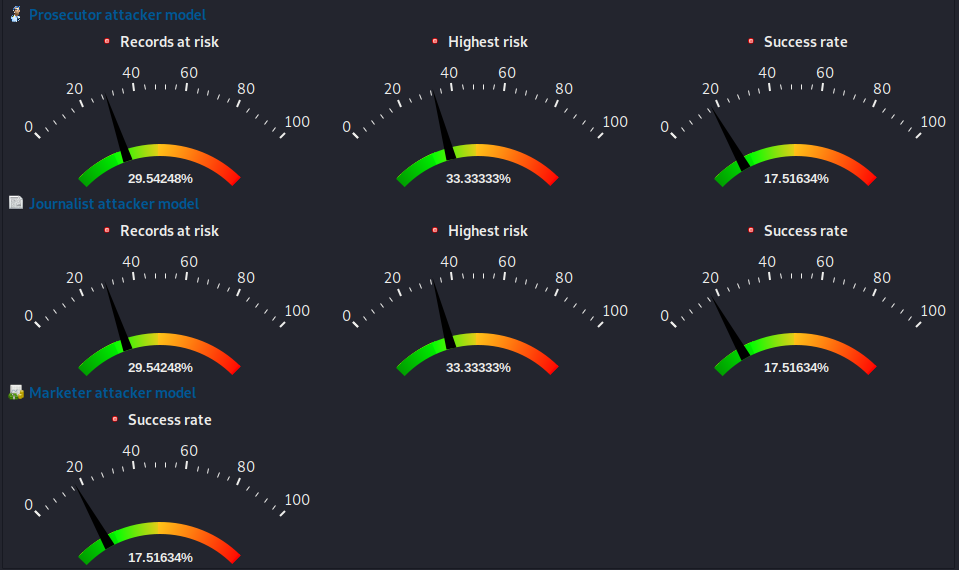
\includegraphics[width=.9\textwidth]{img/risk-model3.png}
	\caption{Risk analysis for \texttt{Model 3}}
	\label{fig:model3-risk}
\end{figure}

\pagebreak

\subsection{Comparative Analysis}

After applying the different privacy models described previously, it is clear 
that the process of anonymizing a dataset should be an \uline{iterative} one. 
As a matter of fact, we had to consistently change parameters in the privacy 
model in order to achieve an acceptable anonymized dataset that could not only 
answer the questions intended, but also have a low risk of re-identification. 
This process is not straight forward or intuitive due to all objectives 
considered. 

Considering the values for the re-identification risk and data utility 
presented previously and summarized in Tables \ref{tab:comparative-analysis} 
and \ref{tab:comparative-risk}, we can see that the first model we considered, 
\texttt{Model 1}, despite maintaining a considerable level of privacy, it does 
not meet the utility requirements. As such, we considered a new privacy model, 
\texttt{Model 2}, that, even though it meets the privacy requirements, too much 
information is lost in the process. This lead us to consider a third privacy 
model, \texttt{Model 3}, that has both an acceptable level of privacy 
protection and data utility.\\

\begin{table}[H]
\centering
\begin{tabular}{c|ccc|}
\cline{2-4}
\textbf{}                                        & 
\multicolumn{3}{c|}{\textbf{Privacy Model}}                 \\ \hline
\multicolumn{1}{|c|}{\textbf{Utility Metric}}               & 
\multicolumn{1}{c|}{\textbf{1}} & \multicolumn{1}{c|}{\textbf{2}} & \textbf{3} 
\\ \hline
\multicolumn{1}{|c|}{\textbf{Number of suppressed records}} & 
\multicolumn{1}{c|}{113}        & \multicolumn{1}{c|}{454}        & 235        
\\ \hline
\multicolumn{1}{|c|}{\textbf{Minimal Class Size}} & \multicolumn{1}{c|}{3}   & 
\multicolumn{1}{c|}{3}    & 3    \\ \hline
\multicolumn{1}{|c|}{\textbf{Average Class Size}} & \multicolumn{1}{c|}{8}   & 
\multicolumn{1}{c|}{4.92} & 5.71 \\ \hline
\multicolumn{1}{|c|}{\textbf{Maximal Class Size}} & \multicolumn{1}{c|}{42}  & 
\multicolumn{1}{c|}{16}   & 27   \\ \hline
\multicolumn{1}{|c|}{\textbf{Number of Classes}}  & \multicolumn{1}{c|}{109} & 
\multicolumn{1}{c|}{111}  & 134  \\ \hline
\end{tabular}
\caption{Comparative analysis of the data utility}
\label{tab:comparative-analysis}
\end{table}

\vspace{\baselineskip}

\begin{table}[H]
\centering
\begin{tabular}{cc|ccc|}
\cline{3-5}
\multicolumn{1}{l}{} &
  \multicolumn{1}{l|}{} &
  \multicolumn{3}{c|}{\textbf{Privacy Model}} \\ \cline{3-5} 
 &
   &
  \multicolumn{1}{c|}{\textbf{1}} &
  \multicolumn{1}{c|}{\textbf{2}} &
  \textbf{3} \\ \hline
\multicolumn{1}{|c|}{\multirow{3}{*}{\textbf{\begin{tabular}[c]{@{}c@{}}Prosecut
or\\ attacker\\ model\end{tabular}}}} &
  \textbf{Records at risk} &
  \multicolumn{1}{c|}{14.43\%} &
  \multicolumn{1}{c|}{39.93\%} &
  29.54\% \\ \cline{2-5} 
\multicolumn{1}{|c|}{} &
  \textbf{Highest risk} &
  \multicolumn{1}{c|}{33.33\%} &
  \multicolumn{1}{c|}{33.33\%} &
  33.33\% \\ \cline{2-5} 
\multicolumn{1}{|c|}{} &
  \textbf{Success rate} &
  \multicolumn{1}{c|}{12.29\%} &
  \multicolumn{1}{c|}{20.33\%} &
  17.51\% \\ \hline
\multicolumn{1}{|c|}{\multirow{3}{*}{\textbf{\begin{tabular}[c]{@{}c@{}}Journali
st\\ attacker\\ model\end{tabular}}}} &
  \textbf{Records at risk} &
  \multicolumn{1}{c|}{14.43\%} &
  \multicolumn{1}{c|}{39.93\%} &
  29.54\% \\ \cline{2-5} 
\multicolumn{1}{|c|}{} &
  \textbf{Highest risk} &
  \multicolumn{1}{c|}{33.33\%} &
  \multicolumn{1}{c|}{33.33\%} &
  33.33\% \\ \cline{2-5} 
\multicolumn{1}{|c|}{} &
  \textbf{Success rate} &
  \multicolumn{1}{c|}{12.29\%} &
  \multicolumn{1}{c|}{20.33\%} &
  17.51\% \\ \hline
\multicolumn{1}{|c|}{\textbf{\begin{tabular}[c]{@{}c@{}}Marketer\\ attacker \\ 
model\end{tabular}}} &
  \textbf{Sucess rate} &
  \multicolumn{1}{c|}{12.29\%} &
  \multicolumn{1}{c|}{20.33\%} &
  17.52\% \\ \hline
\end{tabular}
\caption{Comparative analysis of the re-identification risk}
\label{tab:comparative-risk}
\end{table}

\pagebreak

This being said, the following trends were identified:

\begin{itemize}
    \item Since we considered $k$-anonimity, with $k=3$, the highest risk is
    $1/k = 1/3 \approx 33.33\%$ regardless of other considerations. Values of $k$ 
    greater than this would result in more privacy protection; however, the loss of 
    information would be too excessive.
    \item Constraints on the \texttt{Gender} attribute lead to a considerable 
    number of suppressed records. For example, in \texttt{Model 2}, about 45\% of 
    the records were suppressed.
    \item The constraint on the \texttt{Gender} attribute caused the average 
    equivalence class size of the anonymized dataset to reduce, which, in turn, 
    hinders the privacy protection offered.
\end{itemize}

Overall, considering this pattern, we can safely say that a greater level of 
utility usually implies a lower privacy protection, and vice versa. This 
problem is addressed in Section \ref{sec:privacy-utility-tradeoff}.

It is important to note that this models could be further improved. However, as 
various works have shown, finding the optimal anonymization is a NP-hard 
problem \cite{10.1145/1749603.1749605} and, taking these values into account, 
we consider that \texttt{Model 3} performs reasonably well.

Finally, we also want to point out that we expect that in a larger dataset, the 
re-identification risk would have been smaller given the fact that as the 
number of records increases, more records will have the same value for the 
birth date (\textit{i.e.} this attribute would have a smaller value of 
distinction) and, as such, an attacker who knows the value of this attribute 
for a given record would not have enough information to carry out a record 
linkage attack. This is particularly relevant considering that, as stated in 
Section \ref{sec:risk-analysis}, the birth date uniquely identifies 65.9\% of 
the records. 

\pagebreak

\subsubsection{The Privacy-Utility Trade-off} 
\label{sec:privacy-utility-tradeoff}

In an ideal situation, we'd like to have a dataset with both maximal utility 
and maximal privacy. However, as illustrated in Figure 
\ref{fig:utility_privacy}, such scenario is impossible in the sense that 
maximum privacy means insufficient information utility and, on the other hand, 
maximum utility usually means little to no privacy protection. Indeed, 
\uline{privacy and utility are competing goals}.

In fact, in a real scenario lies in between these two, where the privacy 
protection level is acceptable and the data also retains its utility. In this 
case, we want to make sure that the loss of information is minimal as to 
guarantee that it can still be useful for data analysis. This is particularly 
relevant in the fields of Privacy Preserving Data Mining (PPDM), whose goal is 
to extract knowledge from large amounts of data and provide accurate results 
while preventing sensitive information from disclosure; and Privacy Preserving 
Distributed Data Mining (PPDDM), which allows multiple parties to perform 
collaborative data mining without sharing any piece of data other than the 
final result.\\

\begin{figure}[H]
    \centering
     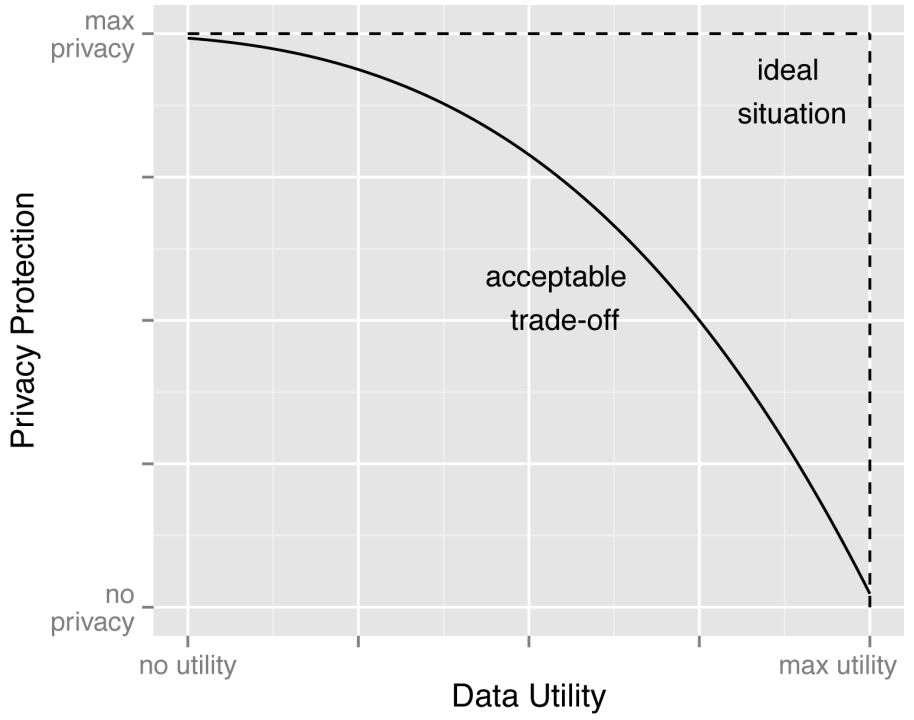
\includegraphics[width=.6\textwidth]{img/privacy-utility.png}
    \caption{Trade-off between \textit{perfect utility} and \textit{perfect 
privacy} \cite{emam2013anonymizing}}
    \label{fig:utility_privacy}
\end{figure}

\pagebreak

\section{Conclusion} \label{sec:conclusion}

In this assignment, we have applied different privacy models and analyzed 
different anonymization techniques in an attempt to reduce the 
re-identification risk while maintaining an acceptable data utility level. In 
doing so, we were able to better understand the differences between privacy 
models and how it affects trade-off between privacy protection and data 
utility. In addition, we were able to conclude that the best privacy model to 
apply to a given dataset is highly dependent on the goal with which we release 
it.

As future work, we would like to try other privacy models such as $LKC$-privacy 
and $(\epsilon, \delta)$-differential privacy, as well as other utility 
metrics, such as information loss and discernability. This would allow us to 
have a clear understanding of the advantages and weaknesses of each privacy 
models. We would also like to experiment with other datasets to see how these 
results would generalise to high-dimensional datasets.

\pagebreak

\bibliographystyle{IEEEtran}
\bibliography{refs}

\pagebreak

\appendix

\section{Data Generation using \texttt{Faker}}

\begin{lstlisting}[language=Python, caption={Python script used to generate 
random synthetic data}, label={lst:faker}]
#!/usr/bin/env python3

import datetime
import pandas as pd
from faker import Faker
from city_state_dic import city_to_state_dict
from random import randrange

fake = Faker()
Faker.seed(42)

# Read the CSV file
df = pd.read_csv('StudentsPerformance.csv')
# Create name, SSN, birth date & city columns
df['name'] = [fake.name() for _ in range(1000)]
df['ssn'] = [fake.ssn() for _ in range(1000)]
df['birth date'] = [fake.date_between_dates(
    date_start=datetime.date(2002, 1, 1),
    date_end=datetime.date(2005, 1, 1)) for _ in range(1000)]
df['city'] = [list(city_to_state_dict.keys())[randrange(2361)]
              for _ in range(1000)]

# Create the average score column and drop the other scores
df['average score'] = ((df['math score'] +
                       df['reading score'] +
                       df['writing score']) / 3).astype(int)

df = df.drop('math score', axis=1)
df = df.drop('reading score', axis=1)
df = df.drop('writing score', axis=1)
df = df.drop('lunch', axis=1)

# Save the CSV file
df.to_csv('StudentsPerformanceUS.csv', encoding='utf-8',
          index=False)
\end{lstlisting}  

\section{Generalization of the \texttt{City} attribute}


\begin{lstlisting}[language=Python, caption={Python script used to replace each 
city with the corresponding State}, label={lst:city-state}]
#!/usr/bin/env python3
import pandas as pd

# city_to_state_dict is a Map with city:state
from city_state_dic import city_to_state_dict

# Read the CSV file
df = pd.read_csv('StudentsPerformanceUS.csv')

# Change each row to the corresponding state
for index, row in df.iterrows():
    df.city[index] = city_to_state_dict[df.city[index]]

# Save the CSV file
df.to_csv('StudentsPerformanceUS-CSG.csv', encoding='utf-8',
          index=False)    
\end{lstlisting}

\end{document}
